\section{Experiments}

During development, the Discovery Service and Specification Retriever software were tested separately by mocking other elements in the Cloudify cluster. This section describes the experiments and their set-ups used to verify that different components integrate and work together flawlessly in a full environment built on real machines. The components in question are the aforementioned Discovery Service and Specification Retriever in addition to Host-Pool Service, Cloudify Manager, Host-Pool Plugin and the test workload, Cloudify Nodecellar Example\cite{Nodecellar}.

\subsection{Hardware set-up}
To verify that the Discovery Service and the Specification retriever function correctly in real environment and on real machines, I set up a test-bed depicted in figure ~\ref{fig:network-venn}.

 \begin{figure}[ht!]
\centering
  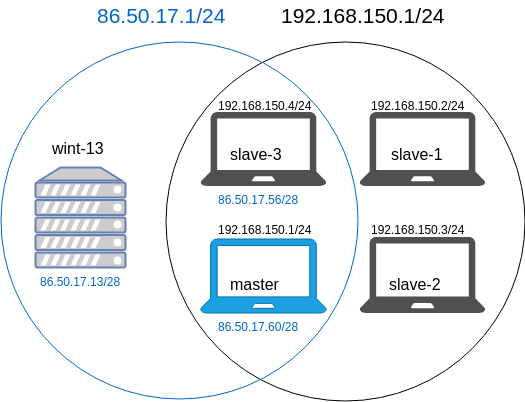
\includegraphics[width=12cm,height=12cm, keepaspectratio]{Network-venn.png}%
  \caption{The testbed hosts are located in a private network but master and slave-3 can also access internet via bastion host wint-13}
  \label{fig:network-venn}
\end{figure}

The test-bed consist of a Lenovo Thinkpad T420S 4173L7G laptop computer with  4-core Intel i5-2540M CPU and 8 GB of RAM acting as a master node in the Cloudify cluster. The three slave-machines are Lenovo Thinkpad Edge E145's with 2-core AMD E1-2500 APU CPUs and 4 GB of RAM. The master host has Centos 7 installed as the operating system to accommodate Cloudify's installation requirements. The three slave machines are running Ubuntu 16.04 as the OS of the slaves can be anything as long as they are Linux-based and the hosts themselves can be accessed via SSH.

\begin{figure}
\centering
  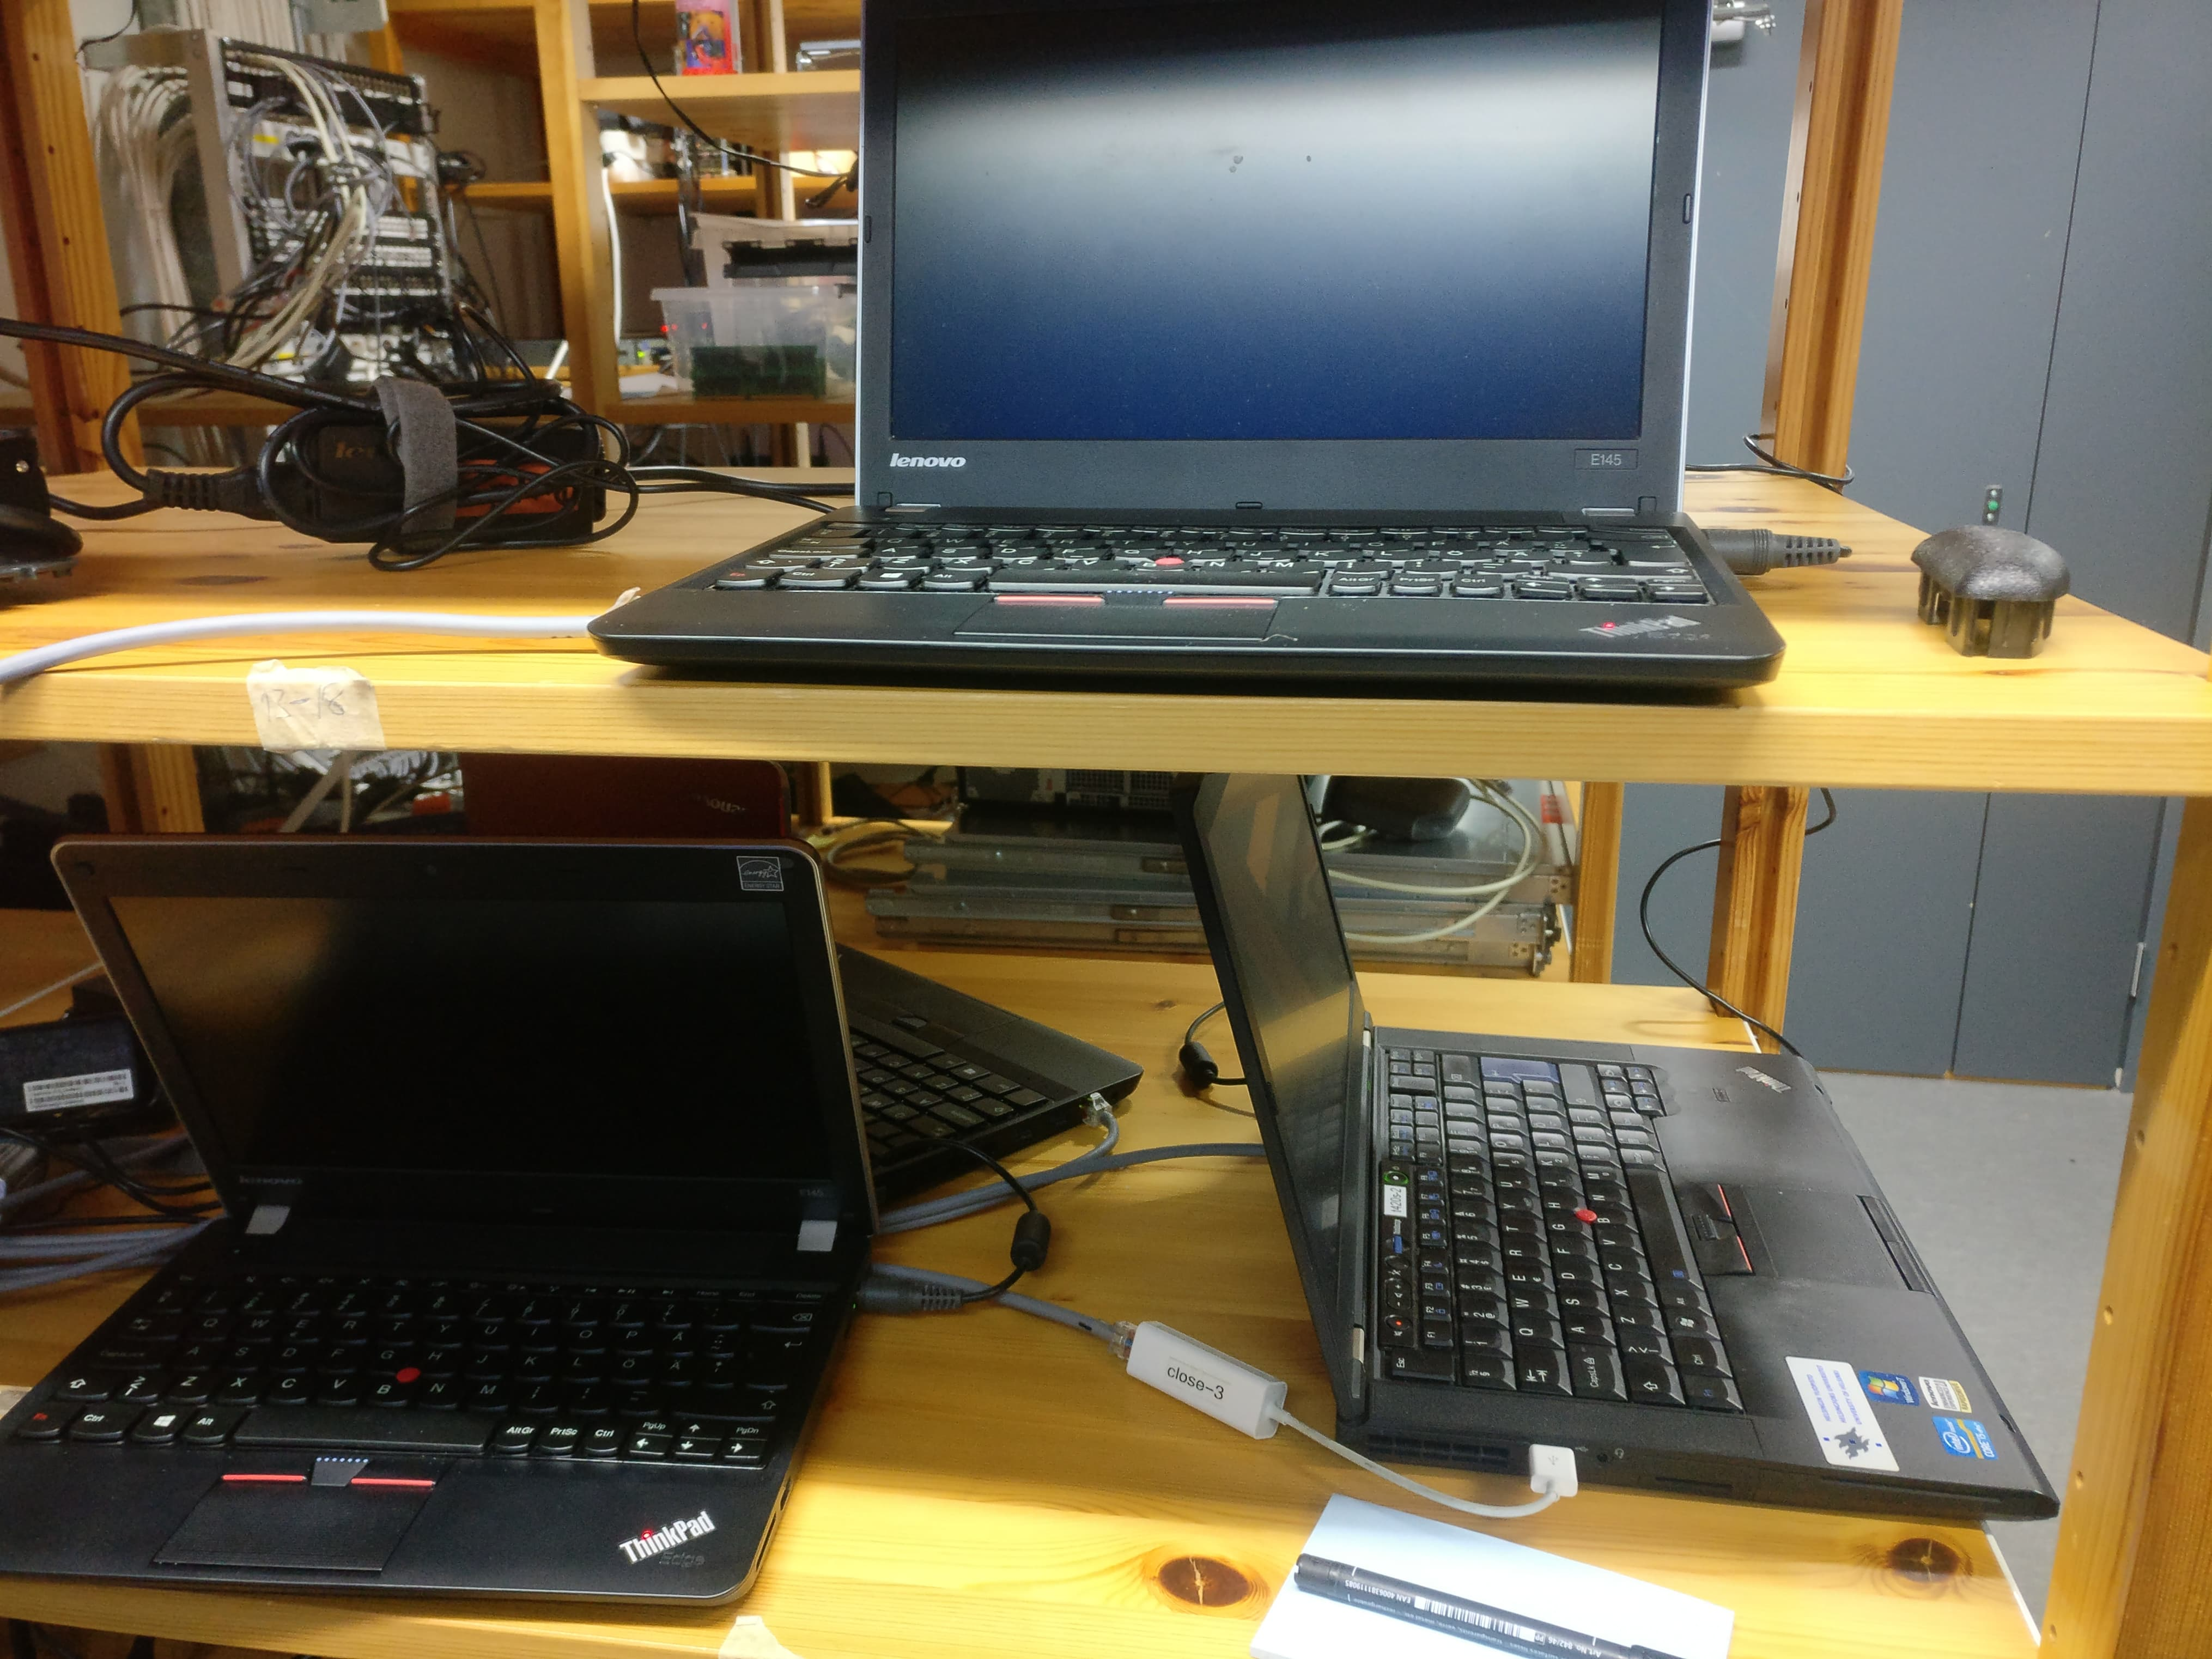
\includegraphics[width=12cm,height=12cm, keepaspectratio]{testbed.jpg}%
  \caption{The actual test-bed. Master node on lower shelf on the right, slaves in the upper and lower shelf}
  \label{fig:test-bed}
\end{figure}

As seen on figure ~\ref{fig:network-venn}, the test-bed set up has two different networks. The Master can be accessed remotely via a bastion host \textit{wint-13}. Wint-13 itself is not a part of the test-bed set up, but it is used to access the testbed remotely and allow internet access for the master host.

Master host has two network interfaces configure for each network it's a part of: The subnet 83.50.17.1 for outside access and 192.168.150.1 which is the subnet dedicated for the Cloudify cluster. Master also serves as a default gateway for all of the slaves. Figure ~\ref{fig:network-venn} shows how slave machines are part of the cluster subnet with static IP addresses. In addition slave-3 is also connected to the 83.50.17.1 subnet. This is to provide a way to drop the host off and connect it back the cluster network but still be able to access it remotely via external network. The physical network is wired with Ethernet cables connected to an HP 5412 zl V2 switch.

\subsection{Software environment set-up}

As mentioned previously, slave hosts do not have many software requirements besides running a Linux distribution as an operating system and having an SSH server installed and accepting connections on the standard port 22. In the test-bed they also have their IP addresses and network interfaces configured statically.

Master node is more intricate than slaves in addition to being more powerful. It has the similar requirements to slaves when it comes to SSH server, but additionally it also runs the following programs:

\begin{itemize}
\item Cloudify Manager
\item Host-pool Plugin within Cloudify Manager
\item Modified Host-pool Service containing Specification Retriever
\item Discovery service
\item Docker
\item Redis running in a Docker container
\end{itemize}

\begin{wraptable}{r}{8cm}
\centering
\begin{tabular}{ | l | p{2cm} | }
\hline
Application & Port \\
\hline
\multicolumn{2}{|c|}{Cloudify ports} \\
\hline
Rest API and UI, HTTP & 80 \\
Rest API and UI, HTTPS & 443 \\
RabbitMQ & 5671 \\
Internal REST communication & 53333 \\
\hline
\multicolumn{2}{| c |}{Other ports} \\
\hline
SSH & 22 \\
Host-pool Service* & 5000 \\
Redis* & 6379 \\
\hline
\multicolumn{2}{| l |}{\textit{* Only internal access}} \\
\hline
\end{tabular}
%\begin{framed}
\caption{Required open ports on the master node. All ports are TCP}
%\end{framed}
\label{table:ports}
\end{wraptable}

In addition the master host has to expose a certain number of ports both internally and externally listed on table ~\ref{table:ports}.

Host-pool plugin runs as a Cloudify deployment managed by Cloudify manager. The modified Host-pool Service runs as a stand-alone Python program listening to port 5000. Even though Cloudify documentation recommends running Host-pool Service as a Cloudify Deployment on a separate host from Cloudify Manager, there are no drawbacks in this kind of local deployment either. 

The Discovery Service is also run as standalone program and it doesn't reserve any ports. However the key-value storage the Discovery Service uses, Redis, is run in a docker container using the official Redis docker image. It reserves the standard  Redis port 6379.

Finally, the server clocks on master host and slave-3 are synchronized with ntp against the ntp servers at \verb|fi.pool.ntp.org| as synchronized time is needed for accurate measurement results in experiment ~\ref{joining_host}.
  

\subsection{Test cases}

To verify that different parts of the Discovery Service and Specification Retriever work in the real environment, I have come up with five test cases which test how different parts of the software integrate with a real system. First three of the test cases test Discovery Service's ability to monitor  the cluster network and deliver the current cluster status to the Host-pool Service. The fourth test verifies that the Specification Retriever script in the modified Host-pool service collects the hardware data correctly. Finally I am going to run an example workload in the cluster which uses the Discovery Service to manage its logical host-pool. This verifies that the system can be used as an addition to a real Cloudify cluster.

The time measurements from all of the applicable test cases are displayed in table ~\ref{table:measurements}. The table shows the fastest and slowest measured times, average and median times as well as standard deviation. Detailed report of the measurement results can be found in appendix ~\ref{testMeasurements}.

\begin{table}
\centering
\begin{tabular}{ | l || l | l | l | l | l |}
\hline 
Test-case \& Time & Fastest & Slowest & Average & Median & Standard Deviation \\
\hline \hline
Start-up & Some time here & Some other time \\
\hline
Joining host \\
\hline
Parting host \\
\hline
Patching a host \\
\hline
\end{tabular}
\caption{Summary of measurements performed in the test cases}
\label{table:measurements}
\end{table}

\subsubsection{Discovering hosts at start up}

As detailed in the section ~\ref{startup}, when Discovery Service is initialised it flushes all of the databases and performs an ARP scan for every IP address in the network. In this experiment I have modified the ARP scanning routine so that it measures the time it takes to scan through the 256 address network. The test is run ten times and the correctness of the scan is checked and the time to completion is measured.

\subparagraph{Results}

\subsubsection{Detecting a joining host} \label{joining_host}

One of the main features of the Discovery Service is the ability to detect machines joining the network in real time. In this test case slave-3 is not initially connected to the cluster network. I have prepared a script which first returns a current timestamp on slave-3 and then enables the network interface facing the cluster network. The sniffer algorithm on the Discovery Service is modified so that it too returns a timestamp upon detecting  a new host. As both hosts are synced against the same time server, the timestamps are comparable allowing me to measure a time it takes for Discovery Service to detect a host after it has joined the network.

\subparagraph{Results}

\subsubsection{Detecting a parted host}

\subparagraph{Results}

\subsubsection{Patching a host}

\subparagraph{Results}

\subsubsection{Retrieving hardware data from the hosts}

Check examples of other cloud providers. Maybe even a table.

\subparagraph{Results}

\subsubsection{Running an example workload in the system}

\subparagraph{Results}